\chapter{Current Mirrors and Current Sources}
Current mirrors are circuits that are used primarily in integrated circuits to bias other circuit elements or act as active loads (such as in the actively loaded differential pair).
They can also be used to sense a current signal in a circuit and mirror (or multiply) it elsewhere to be acted upon or measured by other circuitry.
Current mirrors are commonly constructed out of bipolar transistors or MOSFETs.
They do not find much use outside of integrated circuits because they require transistor matching and sizing (which is easily accomplished when transistors are manufactured in the same \ac{ic} process) and because they usually require less die area than a resistor to provide a particular bias current.

Current mirrors have several important parameters, including current gain, output resistance $R_{o}$ (ideally infinite), systematic gain error $\epsilon$ (deviation from the ideal current gain), and minimum input and output voltages.

\section{Simple current mirror (Bipolar and MOS)}
\begin{center}
	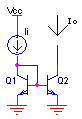
\includegraphics{schematics/simplecurrentmirror.PNG}
\end{center}
This is the most basic form of current mirror.
The two transistors have the same $V_{BE}$ drop (or $V_{GS}$ in the MOS case) since their bases/gates are tied together and their emitters/sources are both connected to a supply voltage or ground.
$Q_1$/$M_1$ is diode connected, which means that the base/gate is shorted to the collector/drain.
\subsection{Bipolar}
For the bipolar case,

\begin{equation}
V_{BE1} = V_{T}\ln\frac{I_{C1}}{I_{S1}} = V_{BE2} = V_{T}\ln\frac{I_{C2}}{I_{S2}}
\end{equation}

(where $I_{S1}$ and $I_{S2}$ are the transistors' saturation currents and $V_{T} = \frac{kT}{q}$ is the thermal voltage).
Canceling terms on both sides, we see that

\begin{equation}
I_{O} = I_{C2} = \frac{I_{S2}}{I_{S1}}I_{C1}
\end{equation}

Assuming $Q_1$ and $Q_2$ have the same $\beta_{F}$, we also know that

\begin{equation}
I_{I} = I_{C1} + \frac{I_{C1}}{\beta_{F}} + \frac{I_{C2}}{\beta_{F}}
\end{equation}

Solving for $I_{C1}$ and substituting we find

\textcolor{red}{
\begin{equation}
I_{O} = \left(\frac{1}{1+\frac{1+(I_{S2}/I_{S1})}{\beta_{F}}}\right)\left(\frac{I_{S2}}{I_{S1}}\right)I_{I}
\label{eq:simplecurrentmirror}
\end{equation}
}

If $I_{S1} = I_{S2}$ the above equation simplifies to

\textcolor{red}{
\begin{equation}
I_{O} = \left(\frac{1}{1 + \frac{2}{\beta_{F}}}\right)I_{I}
\label{eq:simplecurrentmirror_Is_equal}
\end{equation}
}

If $\beta_{F}$ is large the above equations simplify to

\textcolor{red}{
\begin{equation}
I_{O} \approx \frac{I_{S2}}{I_{S1}}I_{I}
\label{eq:simplecurrentmirror_Beta_large}
\end{equation}
}

A bipolar transistor's saturation current $I_{S}$ is proportional to its emitter area so the current gain of the current mirror can be any rational number -- unity, or less than or greater than unity.
The current mirror gets its name from the fact that $I_{C1}$ is mirrored to $I_{C2}$ when the current gain is unity.
One way to set the emitter area ratio when the current gain is not unity is to connect $M$ unit bipolar transistors in parallel as $Q_2$ and $N$ unit bipolar transistors in parallel as $Q_1$ for an emitter area ratio of $M/N$.

The above approximation is the ideal current gain of the current mirror.
Clearly the approximation is not realized (at least in the bipolar case) due to finite $\beta_{F}$.
However, the above analysis neglected the dependence of the transistors' collector currents on the collector-emitter voltage.
Taking into account this dependence as well, the transfer function is

\textcolor{red}{
\begin{equation}
I_{O} = \frac{1+\frac{V_{CE2}-V_{CE1}}{V_{A}}}{1+\frac{1+I_{S2}/I_{S1}}{\beta_{F}}}\frac{I_{S2}}{I_{S1}}I_{I}
\label{eq:fullsimplecurrentmirror}
\end{equation}
}

where $V_{A}$ is the Early voltage.
The systematic gain error is therefore

\textcolor{red}{
\begin{equation}
\epsilon = \frac{1+\frac{V_{CE2}-V_{CE1}}{V_{A}}}{1+\frac{1+I_{S2}/I_{S1}}{\beta_{F}}}-1
\label{eq:simplecurrentmirror_sysgainerr}
\end{equation}
}

and is thus caused by both finite $\beta_{F}$ and finite output resistance $r_{o} = \frac{V_{A}}{I_{C}}$.

The input voltage $V_{I}$ is simply

\textcolor{red}{
\begin{equation}
V_{I} = V_{CE1} = V_{BE1}
\label{eq:simplecurrentmirror_Vi}
\end{equation}
}

since $Q_1$ is diode connected, and the minimum output voltage is

\textcolor{red}{
\begin{equation}
V_{O(\text{min})} = V_{CE2(\text{sat})}
\label{eq:simplecurrentmirror_Vo}
\end{equation}
}

since $Q_2$ must remain in the forward active region.

Another important characteristic of a current mirror is its output resistance.
Ideally, its output resistance is infinite since the current mirror is a current source.
Of course, no real current mirror has an infinite resistance -- in reality the output resistance is dependent on the output current.
For the bipolar case the output resistance \autocite[255-256]{analysis-design-analog-ics} $R_{o}$ is

\textcolor{red}{
\begin{equation}
R_{o} = r_{o2} = \frac{V_{A}}{I_{C2}} = \frac{V_{A}}{I_{O}}
\label{eq:simplecurrentmirror_Ro}
\end{equation}
}

\subsection{MOS}
The MOS current mirror has the same topology as the bipolar current mirror, and its analysis is similar. The MOSFETs must be biased so that $V_{GS} > V_{t}$ (where $V_{t}$ is the threshold voltage).
Using the characteristic equation of a MOSFET in the active region and noting that $V_{GS1} = V_{GS2}$ we see that

\begin{equation}
V_{GS1} = V_{t} + \sqrt{\frac{2I_{D1}}{k'(W/L)_{1}}} = V_{GS2} = V_{t} + \sqrt{\frac{2I_{D2}}{k'(W/L)_{2}}}
\end{equation}

Canceling terms on both sides we see that

\textcolor{red}{
\begin{equation}
I_{O} = \frac{(W/L)_{2}}{(W/L)_{1}}I_{D1} = \frac{(W/L)_{2}}{(W/L)_{1}}I_{I}
\label{eq:MOSsimplecurrentmirror}
\end{equation}
}

As with the bipolar case, the current gain can be set to any rational number by sizing the MOSFETs appropriately. \autocite[258]{analysis-design-analog-ics}

Similar to the bipolar case, the above analysis neglects the slight dependence of a MOSFET's $I_{D}$ to its $V_{DS}$.
If we take this dependency into account, the transfer function is

\textcolor{red}{
\begin{equation}
I_{O} = \frac{(W/L)_{2}}{(W/L)_{1}}I_{I}\left(1+\frac{V_{DS2}-V_{DS1}}{V_{A}}\right)
\label{eq:MOSsimplecurrentmirrorfull}
\end{equation}
}

where $V_{A} = 1/\lambda$, the MOS equivalent of the Early voltage.
The systematic gain error is therefore

\textcolor{red}{
\begin{equation}
\epsilon = \frac{V_{DS2}-V_{DS1}}{V_{A}}
\label{eq:MOSsimplecurrentmirror_sysgainerr}
\end{equation}
}

The input voltage $V_{I}$ is simply

\textcolor{red}{
\begin{equation}
V_{I} = V_{DS1} = V_{GS1}
\label{eq:MOSsimplecurrentmirror_Vi}
\end{equation}
}

since $M_1$ is diode connected, the minimum output voltage $V_{O(min)}$ is

\textcolor{red}{
\begin{equation}
V_{O(min)} = V_{ov2} = \sqrt{\frac{2I_{O}}{(W/L)_{2}k}}
\label{eq:MOSsimplecurrentmirror_Vo}
\end{equation}
}

where $V_{ov}$ is the overdrive voltage above $V_{t}$ (i.e. $V_{GS} = V_{t} + V_{ov}$).
The output resistance $R_{o}$ is \autocite[256, 259]{analysis-design-analog-ics}

\textcolor{red}{
\begin{equation}
R_{o} = r_{o2} = \frac{1}{\lambda I_{D2}} = \frac{1}{\lambda I_{O}}
\label{eq:MOSsimplecurrentmirror_Ro}
\end{equation}
}

For all current mirrors, the current source $I_{I}$ can be implemented by a number of devices.
The simplest is a resistor.
In that case, use the desired $I_{C1}$ and $I_{C2}$ (or $I_{D1}$ and $I_{D2}$ in the MOS case) to determine $V_{BE1} = V_{CE1}$ (or $V_{GS1} = V_{DS1}$) from the transistor's characteristic equation, and then use \ac{kvl} to find $R = \frac{V_{CC} - V_{CE1}}{I_{C1}}$ (or $R = \frac{V_{DD} - V_{DS1}}{I_{D1}}$).

One very useful aspect of current mirrors is that $Q_1$ (or $M_1$) can be used to generate as many output currents as needed;
for each output current simply add another transistor whose base (or gate) is tied to the base (or gate) of $Q_1$ (or $M_1$) and whose emitter (or source) is tied to the emitter (or source) of $Q_1$ (or $M_1$).
The additional output currents flow into the collectors (or drains) of these additional transistors and, by choosing the emitter areas or W/L ratios appropriately, the additional output currents can all have different values.

\section{Simple current mirror with $\beta_{F}$ helper}
\begin{center}
	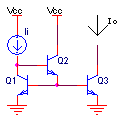
\includegraphics{schematics/currentmirrorbetahelper.PNG}
\end{center}
For the bipolar simple current mirror we assumed $\beta_{F}$ was large enough that we could approximate $I_{O} = \frac{I_{S2}}{I_{S1}}I_{I}$ (the MOS current mirror has an approximately infinite $\beta_{F}$ so it is not applicable here).
To make the current mirror better approximate this ideal relationship (especially if $\beta_{F}$ is relatively small) an additional transistor is added. In this case, \ac{kcl} at $Q_1$'s collector yields

\begin{equation}
I_{I} = I_{C1} + I_{B2}
\label{eq:currentmirrorbetahelper_KCL}
\end{equation}

To find $I_{B2}$ note that

\begin{equation}
I_{E2} = \frac{I_{C1}}{\beta_{F}} + \frac{I_{C3}}{\beta_{F}}
\label{eq:currentmirrorbetahelper_Ie2}
\end{equation}

and

\begin{equation}
I_{B2} = \frac{I_{E2}}{\beta_{F} + 1}
\label{eq:currentmirrorbetahelper_Ib2}
\end{equation}

so substituting (\ref{eq:currentmirrorbetahelper_Ie2}) into (\ref{eq:currentmirrorbetahelper_Ib2}) we have

\begin{equation}
I_{B2} = \frac{I_{C1} + I_{C3}}{\beta_{F}(\beta_{F} + 1)}
\label{eq:currentmirrorbetahelper_Ib2_2}
\end{equation}

Also,

\begin{equation}
I_{C1} = \frac{I_{S1}}{I_{S3}}I_{C3} = \frac{I_{S1}}{I_{S3}}I_{O}
\label{eq:currentmirrorbetahelper_Ic1}
\end{equation}

as before.
Substituting (\ref{eq:currentmirrorbetahelper_Ib2_2}) and (\ref{eq:currentmirrorbetahelper_Ic1}) into (\ref{eq:currentmirrorbetahelper_KCL}) we see

\begin{equation}
I_{I} = \frac{I_{S1}}{I_{S3}}I_{O} + \frac{I_{C1} + I_{C3}}{\beta_{F}(\beta_{F} + 1)} = \frac{I_{S1}}{I_{S3}}I_{O} + \frac{\frac{I_{S1}}{I_{S3}}I_{O} + I_{O}}{\beta_{F}(\beta_{F} + 1)}
\end{equation}

Solving for $I_{O}$ we see that

\textcolor{red}{
\begin{equation}
I_{O} = \left(\frac{1}{1 + \frac{1 + (I_{S3}/I_{S1})}{\beta_{F}(\beta_{F} + 1)}}\right)\frac{I_{S3}}{I_{S1}}I_{I}
\label{eq:currentmirrorbetahelper}
\end{equation}
}

which is the same as the simple current mirror except for the extra $\beta_{F} + 1$ term which multiplies with $\beta_{F}$.

The approximation that

\textcolor{red}{
\begin{equation}
I_{O} \approx \frac{I_{S3}}{I_{S1}}I_{I}
\label{eq:currentmirrorbetahelper_approx}
\end{equation}
}

is even better with the $\beta_{F}$ helper.
Since a MOSFET has $\beta_{F} \approx \infty$ the base current error can be completely eliminated if a MOSFET is used as the $\beta_{F}$ helper transistor.

The $\beta_{F}$ helper does not significantly alter the output resistance $R_{o}$ or the minimum output voltage $V_{O(min)}$, but the input voltage is created by the $V_{BE}$ drop of the $\beta_{F}$ helper (or $V_{GS}$ if the $\beta_{F}$ helper is a MOSFET).
Assuming a bipolar $\beta_{F}$ helper, the input voltage is thus

\textcolor{red}{
\begin{equation}
V_{I} = V_{BE1} + V_{BE2}
\label{eq:currentmirrorbetahelper_Vi}
\end{equation}
}

The current mirror with $\beta_{F}$ helper is also better when multiple outputs are needed.
For every extra output another transistor's base must be connected to the base of $Q_{1}$, which increases the gain error due to the finite $\beta_{F}$.
The $\beta_{F}$ helper reduces this gain error for each output by $\beta_{F}+1$.
The cost of the $\beta_{F}$ helper is that $V_{CE1}$ has an extra $V_{BE}$ drop (now $V_{CE1} = V_{BE1}+V_{BE2}$), which can be a limitation if $V_{CC}$ is low. \autocite[261-262]{analysis-design-analog-ics}

\section{Simple current mirror with $\beta_{F}$ helper and degeneration}
\begin{center}
	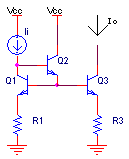
\includegraphics{schematics/currentmirror_betahelper_degeneration.PNG}
\end{center}

\subsection{Bipolar}
Emitter degeneration improves a current mirror by providing better matching between the input current $I_{I}$ and output current $I_{C3}$, and by increasing the mirror's output resistance $R_{o}$ from $R_{o} = r_{o3}$ to

\textcolor{red}{
\begin{equation}
R_{o} \approx r_{o3}(1+g_{m}R_{3})
\end{equation}
}

The increased $R_{o}$ not only makes the current mirror behave more like an ideal current source (which has an infinite $R_{o}$), but it decreases the systematic gain error $\epsilon$ since a finite $R_{o}$ contributes to $\epsilon$.
A simple current mirror with a $\beta_{F}$ helper and emitter degeneration thus has a systematic gain error of

\textcolor{red}{
\begin{equation}
\epsilon = \frac{1+\frac{V_{CE2}-V_{CE1}}{V_{A}(1+\frac{I_{C3}R_{3}}{V_{T}})}}{1+\frac{1+I_{S2}/I_{S1}}{\beta_{F}(\beta_{F}+1)}}-1
\end{equation}
}

The drawback of emitter degeneration is, of course, the increase in the minimum input and output voltages by approximately $I_{I}R_{1}$ and $I_{O}R_{3}$, respectively.
The transfer function is easily expressed in implicit form by using \ac{kvl} and noting that $I_{I} = I_{C1}$ and $I_{O} = I_{C3}$:

\begin{equation}
I_{I}R_{1}+V_{T}\ln\frac{I_{I}}{I_{S1}} = I_{O}R_{3}+V_{T}\ln\frac{I_{O}}{I_{S3}}
\end{equation}

so

\begin{equation}
I_{O} = \frac{1}{R_{3}}\left(I_{I}R_{1} + V_{T}\ln\frac{I_{I}I_{S3}}{I_{O}I_{S1}}\right)
\end{equation}

Given a desired input/output current ratio $\frac{I_{O}}{I_{I}}$, $I_{O}$ can be set by choosing the appropriate resistor ratio $\frac{R_{1}}{R_{3}}$ and/or sizing the transistors appropriately (which changes $\frac{I_{S3}}{I_{S1}}$).

The emitter degeneration resistors are limited by the supply voltage $V_{CC}$ since the input voltage $V_{I}$ is

\textcolor{red}{
\begin{equation}
V_{I} = I_{E1}R_{1}+V_{BE1}+V_{BE2} = \left(\frac{1}{\beta_{F}}+1\right)I_{C1}R_{1}+V_{BE1}+V_{BE2}
\end{equation}
}

and the minimum output voltage $V_{O(min)}$ is

\textcolor{red}{
\begin{equation}
V_{O(\text{min})} = I_{E3}R_{3}+V_{CE3(\text{sat})} = \left(\frac{1}{\beta_{F}}+1\right)I_{C3}R_{3}+V_{CE3(\text{sat})}
\end{equation}
}

and both must be less than $V_{CC}$.
\subsection{MOS}
Source degeneration is not as commonly used as emitter degeneration because matching of MOS current mirrors can be improved by increasing the MOS transistors' gate areas, and $R_{O}$ can be increased by increasing the transitors' channel length.
Nonetheless, the analysis for the bipolar current mirror with $\beta_{F}$ helper and emitter degeneration can be applied to a MOS variant easily. \autocite[262-263]{analysis-design-analog-ics}

\section{Cascode current mirror (Bipolar and MOS)}
\begin{center}
	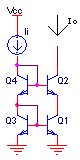
\includegraphics{schematics/cascodecurrentmirror.PNG}
\end{center}

\subsection{Bipolar}
A cascode current mirror significantly increases $R_{o}$.
Transistors $Q_1$ and $Q_3$ in the above schematic form a simple current mirror (which may also include emitter degeneration).
$Q_2$ is in a common base configuration and transfers $I_{C1}$ to $I_{O} = I_{C2}$, and $Q_4$ is connected as a diode to properly bias $Q_2$ and ensure it is in the forward active region.
$R_{o}$ is greatly increased over the simple current mirror (even with emitter degeneration) because the ``emitter resistance'' is the resistance looking into the collector of $Q_1$.
Small-signal analysis reveals that

\textcolor{red}{
\begin{equation}
R_{o} \approx \frac{\beta_{F} r_{o2}}{2}
\end{equation}
}

($R_{o}$ is reduced by half due to the simple current mirror formed by $Q_1$ and $Q_3$, which diverts half of $I_{O} = I_{C2}$ through $r_{\pi 2}$). \autocite[264]{analysis-design-analog-ics}
The drawback of the cascode current mirror versus a simple current mirror is that the input voltage is increased to

\textcolor{red}{
\begin{equation}
V_{I} = V_{BE3} + V_{BE4}
\end{equation}
}

and the minimum output voltage is increased to

\textcolor{red}{
\begin{equation}
V_{O(\text{min})} = V_{BE1} + V_{CE(\text{sat})}
\end{equation}
}

so that both $Q_1$ and $Q_2$ are in the forward active region.

To derive the cascode current mirror's transfer function we note that

\begin{equation}
I_{E4} = I_{C3}+\frac{2I_{C3}}{\beta_{F}}
\label{eq:cascodecurrentmirror_Ie4}
\end{equation}

\begin{equation}
I_{I} = I_{E4}+\frac{I_{C2}}{\beta_{F}}
\label{eq:cascodecurrentmirror_Ii}
\end{equation}

\begin{equation}
I_{O} = I_{C2} = \frac{\beta_{F}}{\beta_{F} + 1}I_{C3}
\label{eq:cascodecurrentmirror_Io}
\end{equation}

Substituting (\ref{eq:cascodecurrentmirror_Ie4}) into (\ref{eq:cascodecurrentmirror_Ii}) we find

\begin{equation}
I_{I} = I_{C3} + \frac{2I_{C3}}{\beta_{F}} + \frac{I_{C3}}{\beta_{F} + 1}
\label{eq:cascodecurrentmirrorIi_2}
\end{equation}

Rearranging (\ref{eq:cascodecurrentmirrorIi_2}) to solve for $I_{C3}$ and substituting the result into (\ref{eq:cascodecurrentmirror_Io}), we see that

\textcolor{red}{
\begin{equation}
I_{O} = \frac{\beta_{F}}{\beta_{F} + 1}\frac{I_{I}}{1+ \frac{2}{\beta_{F}} + \frac{1}{\beta_{F} + 1}} = I_{I}\left(1-\frac{4\beta_{F} + 2}{\beta_{F}^{2} + 4\beta_{F} + 2}\right)
\end{equation}
}

The systematic gain error is clear from the above transfer function:

\textcolor{red}{
\begin{equation}
\epsilon = -\frac{4\beta_{F} +  2}{\beta_{F}^{2} + 4\beta_{F} + 2} \approx -\frac{4}{\beta_{F} + 4}
\end{equation}
}

and is generally greater than $\epsilon$ for a simple current mirror.

\subsection{MOS}
The MOS version of the cascode current mirror does not have the same finite $\beta_{F}$ problems as the bipolar version.
Consequently, a MOS cascode current mirror can be made to have as high an output resistance as needed by increasing the number of stacked cascode MOSFETs (provided the increase in the minimum input and output voltages required by the additional cascodes is acceptable).
The output resistance for a single MOS cascode current mirror is

\textcolor{red}{
\begin{equation}
R_{o} = r_{o2}(1+(g_{m2}+g_{mb2})r_{o1})+ r_{o1}
\end{equation}
}

and each cascode increases $R_{o}$ by approximately a factor of $1+g_{m}r_{o}$ (although in practice $R_{o}$ is limited by parasitic leakage paths as the number of cascodes increases). \autocite[263-268]{analysis-design-analog-ics}
%TODO: Add info on Vo(min) and Vi

\section{Wilson current mirror}
\begin{center}
	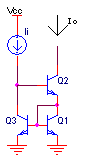
\includegraphics{schematics/wilsoncurrentmirror.PNG}
\end{center}

\subsection{Bipolar}
The Wilson current mirror is a slight variation on the cascode current mirror.
$Q_4$ is removed and $Q_1$ is the only diode connected transistor, which ensures that

\begin{equation}
V_{CE3} = V_{BE1} + V_{BE2} \approx 2V_{BE}
\end{equation}

Bipolar Wilson current mirrors are designed to minimize the systematic gain error $\epsilon$ in cascode current mirrors caused by finite $\beta_{F}$ by using negative feedback through $Q_1$ to activate $Q_3$, which increases $R_{o}$ and reduces the base current error.

To find the transfer function, first use \ac{kcl} at $Q_1$'s collector to find

\begin{equation}
I_{E2} = I_{C1} + I_{B1} + I_{B3} = I_{C1}\left(1+\frac{1}{\beta_{F}}\right) + \frac{I_{C3}}{\beta_{F}}
\end{equation}

Approximating $I_{C1} = I_{C3}$, we see that

\begin{equation}
I_{E2} = I_{C1}\left(1+\frac{2}{\beta_{F}}\right)
\end{equation}

It follows that

\begin{equation}
I_{O} = I_{C2} = I_{E2}\frac{\beta_{F}}{1+\beta_{F}} = I_{C1}\left(1+\frac{2}{\beta_{F}}\right)\left(\frac{\beta_{F}}{1+\beta_{F}}\right)
\label{eq:Wilsoncurrentmirror_Io}
\end{equation}

Finally, substituting

\begin{equation}
I_{C1} = I_{I} - \frac{I_{C2}}{\beta_{F}}
\end{equation}

into (\ref{eq:Wilsoncurrentmirror_Io}) yields

\textcolor{red}{
\begin{equation}
I_{O} = \frac{I_{I}}{1+\frac{2}{\beta_{F} (\beta_{F} + 2)}}
\end{equation}
}

The systematic gain error $\epsilon$ due to finite $\beta_{F}$ is much less than that of the cascode current mirror since there is a $\beta_{F}^{2}$ term.
Note that for simplicity of analysis we have neglected the dependence of $I_{C}$ on $V_{CE}$.

Calculation of the output resistance $R_{o}$ is a bit complicated, so we only give an outline of the derivation here:
apply a test current $i_{t}$ into the output node of the current mirror's small signal model and determine the resulting test voltage $v_{t}$, which gives $R_{o} = \frac{v_{t}}{i_{t}}$.
The small signal model can be simplified by noting that the small signal resistance from the diode connected $Q_{1}$'s base to ground is $1/g_{m1} \parallel r_{\pi1} \parallel r_{\pi3} \parallel r_{o1} \approx 1/g_{m1}$.
Also, $Q_3$ is a voltage controlled current source of magnitude $g_{m3}v_{\pi3} = g_{m3}v_{\pi1} \approx g_{m3}i_{1}/g_{m1} \approx i_{1}$ (where $i_{1}$ is the small signal current through the $1/g_{m1}$ resistance from $Q_1$'s base to ground).
With the model simplified as such, it is easy to see that

\begin{equation}
v_{t} = \frac{i_{i}}{g_{m1}} + (i_{t} - g_{m2}v_{\pi2})r_{o2}
\label{eq:Wilsoncurrentmirror_vt}
\end{equation}

\ac{kcl} at $Q_3$'s collector and $Q_2$'s emitter gives $i_{1}$ in terms of $i_{t}$, $g_{m1}$, $r_{o3}$, and $r_{\pi2}$, and $v_{\pi2}$ in terms of $i_{t}$, $r_{\pi2}$, $g_{m1}$, $r_{o3}$, and $r_{\pi2}$.
The equations for $i_{1}$ and $v_{\pi2}$ can then be substituted into (\ref{eq:Wilsoncurrentmirror_vt}), and rearranging gives \autocite[274-277]{analysis-design-analog-ics}

\textcolor{red}{
\begin{equation}
R_{O} = \frac{1}{g_{m1}\left(1 + \frac{1+\frac{1}{g_{m1}r_{o3}}}{1+\frac{r_{\pi2}}{r_{o3}}}\right)} + r_{o2} + \frac{g_{m2}r_{\pi2}r_{o2}\left(1+\frac{1}{g_{m1}r_{o3}}\right)}{2 + \frac{r_{\pi2}}{r_{o3}} + \frac{1}{g_{m1}r_{o3}}}
\end{equation}
}

For $r_{o3} \to \infty$, we can simplify the above equation considerably:

\textcolor{red}{
\begin{equation}
R_{O} \approx \frac{1}{2g_{m1}} + r_{o2} + \frac{g_{m2}r_{\pi2}r_{o2}}{2} \approx \frac{\beta_{F} r_{o2}}{2}
\end{equation}
}

Fortunately, the input and minimum output voltages can be determined by inspection: they are

\textcolor{red}{
\begin{equation}
V_{I}= V_{BE1} + V_{BE2} \approx 2V_{BE}
\end{equation}
}

\textcolor{red}{
\begin{equation}
V_{O(\text{min})} = V_{BE1} + V_{CE(\text{sat})}
\end{equation}
}

\subsection{MOS}
The MOS variant is analogous to the bipolar case, except that $\beta_{F} \to \infty$ and $r_{\pi} \to \infty$.
The above analysis for the bipolar case thus suggests that

\textcolor{red}{
\begin{equation}
I_{O} = I_{I}
\end{equation}
}

\textcolor{red}{
\begin{equation}
R_{o} = \frac{1}{g_{m1}}+r_{o2}+g_{m2}r_{o2}\left(1+\frac{1}{g_{m1}r_{o3}}\right)r_{o3} \approx (1+g_{m2}r_{o3})r_{o2}
\end{equation}
}

Since we neglected the dependence of $I_{C}$ on $V_{CE}$ for the analysis of the bipolar Wilson current mirror, we have also neglected the the dependence of $I_{D}$ on $V_{DS}$ for the MOS case.
The systematic gain error $\epsilon$ thus is not zero as the above transfer function would suggest.
Due to the mismatch between $V_{DS1}$ and $V_{DS3}$, the systematic gain error is actually

\textcolor{red}{
\begin{equation}
\epsilon = \frac{V_{DS1}-V_{DS3}}{V_{A}}
\end{equation}
}

The input voltage is simply

\textcolor{red}{
\begin{equation}
V_{I} = V_{GS1}+V_{GS2}
\end{equation}
}

and the minimum output voltage is

\textcolor{red}{
\begin{equation}
V_{O(\text{min})} = V_{GS1}+V_{GS2} = V_{t}+2V_{ov}
\end{equation}
}

where $V_{ov}$ is the overdrive voltage about $V_{t}$.

\section{Improved Wilson current mirror}
\begin{center}
	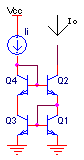
\includegraphics{schematics/wilsoncurrentmirrorimproved.PNG}
\end{center}
The improved Wilson current mirror adds a fourth transistor whose base (or gate) is connected to $Q_2$ (or $M_2$) and is placed in series with $Q_3$ (or $M_3$).
This fourth transistor forces the collector (or drain) voltage of $Q_1$ (or $M_1$) to equal the collector (or drain) voltage of $Q_3$ (or $M_3$) so that $V_{CE1} = V_{CE3}$ (bipolar) and $V_{DS1} = V_{DS3}$ (MOS).
This eliminates the systematic gain error due to the voltage mismatches in the simple Wilson current mirror, thus reducing $\epsilon$ in the bipolar case and eliminating it in the MOS case. \autocite[277-278]{analysis-design-analog-ics}

\subsection{Bipolar}
The characteristic equations of the bipolar improved Wilson current mirror are

\textcolor{red}{
\begin{equation}I_{O} = \frac{I_{I}}{1+\frac{2}{\beta_{F} (\beta_{F} + 2)}}
\end{equation}
}

\textcolor{red}{
\begin{equation}
V_{I}= V_{BE1} + V_{BE2} \approx 2V_{BE}
\end{equation}
}

\textcolor{red}{
\begin{equation}
V_{O(min)} = V_{BE1} + V_{CE(sat)}
\end{equation}
}

\textcolor{red}{
\begin{equation}
\epsilon = \frac{1}{1+\frac{2}{\beta_{F} (\beta_{F} + 2)}}
\end{equation}
}

\textcolor{red}{
\begin{equation}
R_{o} = \frac{1}{g_{m1}\left(1 + \frac{1+\frac{1}{g_{m1}r_{o3}}}{1+\frac{r_{\pi2}}{r_{o3}}}\right)} + r_{o2} + \frac{g_{m2}r_{\pi2}r_{o2}\left(1+\frac{1}{g_{m1}r_{o3}}\right)}{2 + \frac{r_{\pi2}}{r_{o3}} + \frac{1}{g_{m1}r_{o3}}}
\end{equation}
}

The output resistance $R_{o}$ can be approximated as

\textcolor{red}{
\begin{equation}
R_{o} \approx \frac{1}{2g_{m1}} + r_{o2} + \frac{g_{m2}r_{\pi2}r_{o2}}{2} \approx \frac{\beta_{F} r_{o2}}{2}
\end{equation}
}

The only difference is in $\epsilon$, which no longer has a component caused by a mismatch between $V_{CE1}$ and $V_{CE3}$.

\subsection{MOS}
The characteristic equations of the MOS improved Wilson current mirror are

\textcolor{red}{
\begin{equation}
I_{O} = I_{I}
\end{equation}
}

\textcolor{red}{
\begin{equation}
R_{O} = \frac{1}{g_{m1}}+r_{o2}+g_{m2}r_{o2}\left(1+\frac{1}{g_{m1}r_{o3}}\right)r_{o3} \approx (1+g_{m2}r_{o3})r_{o2}
\end{equation}
}

\textcolor{red}{
\begin{equation}
V_{I} = V_{GS1}+V_{GS2}
\end{equation}
}

\textcolor{red}{
\begin{equation}
V_{O(min)} = V_{GS1}+V_{GS2} = V_{t}+2V_{ov}
\end{equation}
}

\textcolor{red}{
\begin{equation}
\epsilon = 0
\end{equation}
}

The only difference is again in $\epsilon$, which in the MOS case is reduced to zero since there is no systematic gain error due to finite $\beta_{F}$, and the systematic gain error due to the mismatch betweeen $V_{DS1}$ and $V_{DS3}$ has been reduced to zero due to the fact that we now have $V_{DS1} = V_{DS3}$.

\section{Sooch cascode current mirror (MOS)}
\begin{center}
	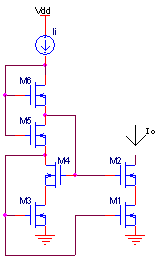
\includegraphics{schematics/soochcascodecurrentmirror.PNG}
\end{center}
The Sooch cascode current mirror is designed to allow a higher output voltage swing by increasing $V_{O(min)}$ at the expense (increase) of $V_{I(min)}$.
Referring back to the single MOS cascode current mirror shown above,

\begin{equation}
V_{DS1} = V_{GS3} + V_{GS4} - V_{GS2} = V_{t} + V_{ov}
\end{equation}

where $V_{ov}$ is the overdrive voltage above the MOSFETs' $V_{t}$ (i.e. $V_{GS} = V_{t} + V_{ov}$).
Since $M_1$ only requires

\begin{equation}
V_{DS1} \geq V_{ov}
\end{equation}

to remain in the active region, the cascode current mirror biases $V_{DS1}$ unnecessarily large.
The Sooch cascode current mirror level shifts $V_{G2}$ down by $V_{t}$ so that

\begin{equation}
V_{DS1} = V_{ov}
\end{equation}

and thus

\textcolor{red}{
\begin{equation}
V_{O(\text{min})} = 2V_{ov}
\end{equation}
}

The necessary level shift is achieved by adding $M_5$ and $M_6$ and rewiring $M_4$ as shown in the above schematic.
First, consider $M_5$ and $M_6$ alone:
$M_6$ is diode connected so it is biased in the active region as long as

\begin{equation}
I_{D6} = I_{I} > 0
\end{equation}

\begin{equation}
V_{GS6} > V_{t}
\end{equation}

A channel exists at the drain of $M_5$ since

\begin{equation}
V_{GS6} = V_{DG5}
\end{equation}

and a channel exists at the source of $M_6$.
$M_5$ is thus biased in the triode region by $M_6$.
We want

\begin{equation}
V_{G2} = V_{GS3} + V_{DS5} = V_{t} + 2V_{ov}
\end{equation}

so that

\begin{equation}
V_{DS1} = V_{G2} - V_{GS2} = (V_{t} + 2V_{ov}) - (V_{t} + V_{ov}) = V_{ov}
\end{equation}

We know

\begin{equation}
V_{GS3} = V_{S5} = V_{t} + V_{ov}
\end{equation}

so we need

\begin{equation}
V_{DS5} = V_{ov}
\end{equation}

We also need

\begin{equation}
V_{GS6} = V_{t} + V_{ov}
\end{equation}

so that $I_{D6}$ is equal to the other drain currents.
Since $M_{5}$ is in the triode region and $M_6$ is in the active region, we know that

\begin{equation}
I_{I} = I_{D5} = I_{D6} = \frac{k'}{2}\left(\frac{W}{L}\right)_{6}(V_{GS6}-V_{6})^{2} = \frac{k'}{2}\left(\frac{W}{L}\right)_{5}(2(V_{GS5}-V_{t})V_{DS5} - V_{DS5}^{2})
\label{eq:Soochcurrentmirror_Ii}
\end{equation}

Substituting

\begin{equation}
V_{GS5} = V_{GS6} + V_{DS5} = V_{t} + 2V_{ov}
\end{equation}

into (\ref{eq:Soochcurrentmirror_Ii}), we have

\begin{equation}
\frac{k'}{2}\left(\frac{W}{L}\right)_{6}V_{ov}^{2} = \frac{k'}{2}\left(\frac{W}{L}\right)_{5}(4V_{ov}^{2}-V_{ov}^{2})
\end{equation}

so we need

\begin{equation}
(\frac{W}{L})_{5} = \frac{1}{3}(\frac{W}{L})_{6}
\end{equation}

$M_4$ is obviously used to ensure that

\begin{equation}
V_{DS1} = V_{DS3}
\end{equation}

to minimize the systematic gain error $\epsilon$.
With $M_4$ connected as shown, we have

\begin{equation}
V_{DS3} = V_{G2} - V_{GS4}
\end{equation}

We designed

\begin{equation}
V_{G2} = V_{t} + 2V_{ov}
\end{equation}

(ignoring channel length modulation) so that

\begin{equation}
V_{O} = 2V_{ov}
\end{equation}

and we know that

\begin{equation}
V_{GS4} = V_{t} + V_{ov}
\end{equation}

(ignoring the body effect and assuming that $M_4$ is in the active region), so we can substitute these equations to find that

\begin{equation}
V_{DS3} = V_{ov}
\end{equation}

$V_{DS3}$ is thus equal to $V_{DS1}$. \autocite[270-273]{analysis-design-analog-ics}
A MOS current mirror does not suffer from finite $\beta_{F}$ so the matched $V_{DS1} = V_{DS3}$ means that

\textcolor{red}{
\begin{equation}
\epsilon = 0
\end{equation}
}

The Sooch cascode current mirror has the same output resistance $R_{o}$ as the simple cascode current mirror since the output transistors are unchanged:

\textcolor{red}{
\begin{equation}
R_{o} = r_{o2}(1+(g_{m2}+g_{mb2})r_{o1})+ r_{o1}
\end{equation}
}

The Sooch cascode current mirror has good $V_{O(min)}$ and $\epsilon$, but the low $V_{O(min)}$ comes at the cost of

\begin{equation}
V_{I(min)} = V_{GS3} + V_{GS5}
\end{equation}

From the above analysis, this gives

\textcolor{red}{
\begin{equation}
V_{I(min)} = 2V_{t} + 3V_{ov}
\end{equation}
}

\section{High-swing current mirror with two input branches}
\begin{center}
	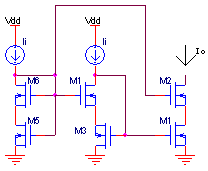
\includegraphics{schematics/highswingcascodecurrentmirror.PNG}
\end{center}
The above Sooch cascode current mirror provides a high output voltage swing using only one input branch at the cost of significantly increasing $V_{I(min)}$.
This circuit also provides a high output voltage swing but uses a second input branch to lower $V_{I(min)}$.
The second input branch increases the current mirror's power consumption since the second branch draws additional current from $V_{DD}$;
in contrast, the added transistors in the Sooch cascode current mirror share the same current as the two transistors of simple cascode current mirror's input branch so they do not increase power consumption.
If $V_{DD}$ is too low or needs to be minimized, however, the increase of $V_{I(min)}$ may prohibit the use of the Sooch cascode current mirror in favor of this circuit.

$M_5$ and $M_6$ are configured the same for this circuit and the Sooch cascode current mirror, so from the above analysis we need

\begin{equation}
\left(\frac{W}{L}\right)_{5} = \frac{1}{3}\left(\frac{W}{L}\right)_{6}
\end{equation}

The minimum input voltage for this circuit is the greater of the two minimum input voltages for each of the input branches.
The left input branch has

\begin{equation}
V_{I(\text{min})} = V_{DS5} + V_{GS6} = V_{t} + 2V_{ov}
\end{equation}

and the right input branch has

\begin{equation}
V_{I(\text{min})} = V_{GS3} = V_{t} + V_{ov}
\end{equation}

Thus, the overall minimum input voltage is \autocite[273]{analysis-design-analog-ics}

\textcolor{red}{
\begin{equation}
V_{I(\text{min})} = V_{t} + 2V_{ov}
\end{equation}
}

As with the Sooch cascode current mirror, the output transistors are unmodified from the simple cascode current mirror so

\textcolor{red}{
\begin{equation}
R_{o} = r_{o2}(1 + (g_{m2} + g_{mb2})r_{o1}) + r_{o1}
\end{equation}
}

\textcolor{red}{
\begin{equation}
V_{O(\text{min})} = 2V_{ov}
\end{equation}
}

\section{Collector current source}
\begin{center}
	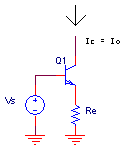
\includegraphics{schematics/collectorcurrentsource.PNG}
\end{center}
This is a very basic current source which uses a voltage source $V_{S}$ and emitter resistor $R_{E}$ to bias a bipolar transistor to the desired collector current $I_{C}$, which is the output of the current source.
The voltage source and $R_{E}$ determine

\begin{equation}
V_{BE} = V_{S} - I_{E}R_{E} = V_{S} - \frac{\beta_{F}+1}{\beta_{F}}I_{C}R_{E}
\end{equation}

where the latter equation results from the relationship between $I_{C}$ and $I_{E}$ defined in (\ref{eq:bipolarIewrtIc}).
Thus, the output current can be expressed in terms of $V_{BE}$ as

\textcolor{red}{
\begin{equation}
I_{C} = \frac{\beta_{F}}{\beta_{F}+1}\frac{V_{S}-V_{BE}}{R_{E}}
\label{eq:collector_currentsource_Ic_wrt_Vbe}
\end{equation}
}

Solving for $V_{BE}$ in (\ref{eq:bipolarIc}) we find

\begin{equation}
V_{BE} = V_{th}\ln\left(\frac{I_{C}}{I_{S}}+1\right)
\end{equation}

so that we can express $I_{C}$ in a transcendental equation

\textcolor{red}{
\begin{equation}
I_{C} = \frac{\beta_{F}}{\beta_{F}+1} \frac{V_{S}-V_{th}\ln\left(\frac{I_{C}}{I_{S}}+1\right)}{R_{E}}
\end{equation}
}

The bipolar transistor is configured the same way as the common emitter, so the output resistance $R_{O}$ can be borrowed from (\ref{eq:commonemitter_Ro}):

\textcolor{red}{
\begin{equation}
R_{o} = \left(\frac{r_{\pi}R_{E}}{r_{\pi}+R_{E}} + r_{o}\left(1+g_{m}\frac{r_{\pi}R_{E}}{r_{\pi}+R_{E}}\right)\right)
\end{equation}
}

The MOS version of the collector current source is the drain current source.
With a source resistor $R_{S}$ the output current $I_{D} = I_{O}$ depends on $V_{GS}$ as

\textcolor{red}{
\begin{equation}
I_{D} = \frac{V_{S}-V_{GS}}{R_{S}}
\label{eq:draincurrentsource_Id_wrt_Vgs}
\end{equation}
}

By rearranging (\ref{eq:activeId}) to solve for $V_{GS}$ and substituting into (\ref{eq:draincurrentsource_Id_wrt_Vgs}) we can express $I_{O}$ as a transcendental equation:

\textcolor{red}{
\begin{equation}
I_{D} = \frac{V_{S}-V_{t}-\sqrt{\frac{L}{W}\frac{2I_{D}}{\mu_{n}C_{ox}}}}{R_{S}}
\end{equation}
}

The MOSFET is configured as a common source so the output resistance $R_{o}$ is

\textcolor{red}{
\begin{equation}
R_{o} = R_{S} + (1+(g_{m}+g_{mb})R_{S})r_{o}+R_{S}
\end{equation}
}

which is borrowed from (\ref{eq:commonsource_Ro}).

\section{Diode connected collector/drain current source}
\begin{center}
	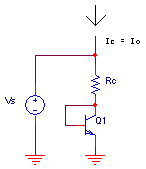
\includegraphics{schematics/diodeconnected_collector_currentsource.PNG}
\end{center}
The diode connected collector current source is similar to the simple collector current source.
\ac{kvl} around the circuit's loop shows that

\begin{equation}
I_{C}R_{C} = V_{S} - V_{CE} = V_{S} - V_{BE}
\end{equation}

Dividing both sides by $R_{C}$ to solve for $I_{C} = I_{O}$ gives

\textcolor{red}{
\begin{equation}
I_{O} = \frac{V_{S}-V_{BE}}{R_{C}}
\end{equation}
}

This is nearly identical to (\ref{eq:collector_currentsource_Ic_wrt_Vbe}), so we can borrow the above analysis to express $I_{O}$ as a transcendental equation:

\textcolor{red}{
\begin{equation}
I_{C} = \frac{V_{S}-V_{th}\ln\left(\frac{I_{C}}{I_{S}}+1\right)}{R_{C}}
\end{equation}
}

The MOS version is the diode connected drain current source. With a drain resistor $R_{D}$ the output current $I_{O} = I_{D}$ is

\textcolor{red}{
\begin{equation}
I_{O} = \frac{V_{S}-V_{GS}}{R_{D}}
\end{equation}
}

Again, we can borrow the above analysis to write $I_{O}$ as a transcendental equation:

\textcolor{red}{
\begin{equation}
\frac{V_{S}-V_{t}-\sqrt{\frac{L}{W}\frac{2I_{D}}{\mu_{n}C_{ox}}}}{R_{D}}
\end{equation}
}

A notable characteristic of this current source is that the output voltage is simply $V_{S}$.

\section{Peaking current source}
\begin{center}
	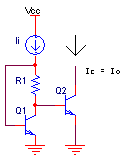
\includegraphics{schematics/peakingcurrentsource.PNG}
\end{center}
The Peaking current source is useful for generating very small currents (e.g., in the nA range) without using large values of resistance.
It is available in bipolar and CMOS technologies with identical topologies but with a slightly different analysis between the bipolar and CMOS versions.

\subsection{Bipolar}
Applying \ac{kvl} and neglecting the small $I_{B1}$ current,

\begin{equation}
V_{BE2} = V_{BE1} - I_{I}R_{1}
\label{eq:peaking_currentsource_KVL}
\end{equation}

Still neglecting the small base currents,

\begin{equation}
I_{C1} = I_{I}
\end{equation}

and, trivially,

\begin{equation}
I_{C2} = I_{O}
\end{equation}

Using (\ref{eq:bipolarIc}) and solving it for $V_{BE}$, we can substitute for $V_{BE1}$ and $V_{BE2}$ in (\ref{eq:peaking_currentsource_KVL}) and substitute $I_{I}$ for $I_{C1}$ and $I_{O}$ for = $I_{C2}$ to find

\begin{equation}
I_{I}R_{1} = V_{T}\ln\left(\frac{I_{I}}{I_{S1}}\right) - V_{T}\ln\left(\frac{I_{O}}{I_{S2}}\right)
\label{eq:peaking_currentsource_transferfunc_first}
\end{equation}

If $Q_1$ and $Q_2$ are identical so that $I_{S1} = I_{S2}$ we can rewrite (\ref{eq:peaking_currentsource_transferfunc_first}) and solve for $I_{O}$ in terms of $I_{I}$:

\textcolor{red}{
\begin{equation}
I_{O} = I_{I}e^{-\frac{I_{I}R_{1}}{V_{T}}}
\end{equation}
}

For a circuit design problem in which $I_{I}$ and $I_{O}$ are determined and the appropriate value of $R_{1}$ must be found, it is useful to know $R_{1}$ in terms of $I_{I}$ and $I_{O}$.
Rewriting (\ref{eq:peaking_currentsource_transferfunc_first}) and again assuming $Q_1$ and $Q_2$ are identical,

\textcolor{red}{
\begin{equation}
R_1 = \frac{V_{T}}{I_{I}}\ln\left(\frac{I_{I}}{I_{O}}\right)
\label{eq:peaking_currentsource_R}
\end{equation}
}

To demonstrate the usefulness of the Peaking current source for generating small currents without requiring large resistors, suppose $I_{I} = \SI{10}{\mu A}$ and $I_{O} = \SI{100}{nA}$.
Also suppose $V_{T} = \SI{26}{mV}$ (the approximate thermal voltage at room temperature).
In that case application of (\ref{eq:peaking_currentsource_R}) shows that the required resistor would be $R_1 \approx \SI{12}{k\ohm}$. \autocite[303-304]{analysis-design-analog-ics}

\subsection{MOS}
The analysis of the MOS Peaking current source is similar. \ac{kvl} shows that

\begin{equation}
V_{GS2} = V_{GS1} - I_{I}R_{1}
\label{eq:MOS_peaking_currentsource_KVL}
\end{equation}

The sources of $M_1$ and $M_2$ are connected together so the threshold voltages $V_{t}$ cancel and (\ref{eq:MOS_peaking_currentsource_KVL}) simplifies to

\begin{equation}
V_{ov2} = V_{ov1} - I_{I}R_{1}
\label{eq:MOS_peaking_currentsource_KVL_Vov}
\end{equation}

where the overdrive voltage $V_{ov}$ is defined as $V_{ov} = V_{GS} - V_{t}$.
Assuming $M_1$ and $M_2$ operate in the active region and strong inversion, we can use (\ref{eq:activeId}) and (\ref{eq:MOS_peaking_currentsource_KVL_Vov}) to find

\begin{equation}
I_{O} = \frac{k'}{2}\left(\frac{W}{L}\right)_{2}V_{ov2}^{2} = \frac{k'}{2}\left(\frac{W}{L}\right)_{2}(V_{ov1}-I_{I}R_{1})^{2}
\label{eq:MOS_peaking_currentsource_Io_strong}
\end{equation}

However, the input current $I_{I}$ is often small enough that $M_1$ must operate in weak inversion and, since $V_{ov2} < V_{ov1}$ from (\ref{eq:MOS_peaking_currentsource_KVL_Vov}), $M_2$ must also operate in weak inversion (where $I_{D}$ is an exponential function of $V_{GS}$).
Assuming $V_{DS1} > 3V_{T}$ and $V_{DS2} > 3V_{T}$ and the transistors are identical, we can apply (\ref{eq:Idweakinversion}) to both transistors and substitute into (\ref{eq:MOS_peaking_currentsource_Io_strong}) to find

\textcolor{red}{
\begin{equation}
I_{O} \approx \frac{W}{L}I_{t}e^{\frac{V_{GS2}-V_{t}}{nV_{T}}} \approx I_{I}e^{\frac{I_{I}R_{1}}{nV_{T}}}
\end{equation}
}

The transfer functions of the bipolar and MOS versions of the Peaking current source are thus nearly the same, with the exception of the multiplicative factor $n$ to the thermal voltage $V_{T}$, where $n$ is defined in (\ref{eq:Id_n}).
For MOS transistors, $1.3 \leq n \leq 1.5$ and effectively $n = 1$ for bipolar transistors. \autocite[304-305]{analysis-design-analog-ics}

\section{$\Delta V_{BE}$ current source (DC Analysis 1)}
\begin{center}
	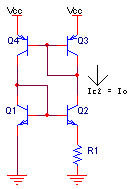
\includegraphics{schematics/deltaVbe_currentsource.PNG}
\end{center}

\section{Base-emitter referenced current source}
\begin{center}
	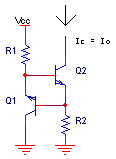
\includegraphics{schematics/base-emitter_referenced_currentsource.PNG}
\end{center}
The base-emitter referenced current source is designed to decrease the sensitivity of the output current $I_{O}$ on the supply voltage $V_{CC}$ by designing $I_{O}$ to depend on a transistor's $V_{BE}$.
Assuming both transistors are biased in the forward active region, the base currents are small and can be neglected so that we can use (\ref{eq:bipolarIc}) solved for $V_{BE}$ to find

\begin{equation}
V_{BE1} = V_{T}\ln\left(\frac{I_{I}}{I_{S1}}\right)
\end{equation}

since

\begin{equation}
I_{C} = I_{I} - I_{B2} \approx I_{I}
\end{equation}

The voltage across $R_2$ is simply $V_{BE1}$ and the current through it is $I_{E2}$ so

\begin{equation}
I_{E2} = \frac{V_{BE1}}{R_2} = \frac{V_{T}}{R_2}\ln\left(\frac{I_{I}}{I_{S1}}\right)
\end{equation}

Again assuming the base currents are negligible

\begin{equation}
I_{O} = I_{C2} = I_{E2} - I_{B2} \approx I_{E2}
\end{equation}

so that

\textcolor{red}{
\begin{equation}
I_{O} = \frac{V_{T}}{R_{2}}ln(\frac{I_{I}}{I_{S1}})
\label{eq:Vbe_reference_current_source}
\end{equation}
}

Since the point of the base-emitter reference current source is to decrease the sensitivity of $I_{O}$ to $V_{CC}$, $S_{{V}_{CC}}^{{I}_{O}}$, it is useful to quantify it.
By definition \autocite[306]{analysis-design-analog-ics},

\begin{equation}
S_{{V}_{CC}}^{{I}_{O}} = \frac{V_{CC}}{I_{O}}\frac{\partial I_{O}}{\partial V_{CC}}
\label{eq:S_Io_to_Vcc}
\end{equation}

so differentiating (\ref{eq:Vbe_reference_current_source}) with respect to $V_{CC}$ and substituting the result into (\ref{eq:S_Io_to_Vcc}) shows that

\begin{equation}
S_{{V}_{CC}}^{{I}_{O}} = \frac{V_{T}}{I_{O}R_{2}}S_{{V}_{CC}}^{{I}_{I}} = \frac{V_{T}}{V_{BE1}}S_{{V}_{CC}}^{{I}_{I}}
\end{equation}

If $V_{CC} \gg V_{BE1} + V_{BE2}$ then $V_{CC}$ is the approximate voltage across $R_{1}$ and

\begin{equation}
I_{I} \approx \frac{V_{CC}}{R_{1}}
\end{equation}

so that $S_{{V}_{CC}}^{{I}_{I}}$ is approximately unity and thus

\textcolor{red}{
\begin{equation}
S_{{V}_{CC}}^{{I}_{O}} \approx \frac{V_{T}}{V_{BE1}}
\end{equation}
}

For typical values of $V_{T}$ and $V_{BE1}$, $S_{{V}_{CC}}^{{I}_{O}}$ is less than ten percent.

\section{Threshold referenced current source}
\begin{center}
	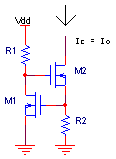
\includegraphics{schematics/threshold_referenced_currentsource.PNG}
\end{center}
The threshold referenced current source is the MOS equivalent to the base-emitter referenced current source.
The output current $I_{O}$ is the current through $R_2$, which has a voltage $V_{GS1}$ across it.
Using (\ref{eq:activeId}) solved for $V_{GS}$ we see that

\textcolor{red}{
\begin{equation}
I_{O} = \frac{V_{GS1}}{R_{2}} = \frac{V_{t} + \sqrt{\frac{2I_{I}}{k'(W/L)_{1}}}}{R_{2}}
\label{eq:threshold_referenced_current_source}
\end{equation}
}

Differentiating (\ref{eq:threshold_referenced_current_source}) with respect to the supply voltage $V_{DD}$ gives the sensitivity $I_{O}$ to $V_{DD}$:

\begin{equation}
S_{{V}_{DD}}^{{I}_{O}} = \frac{V_{ov1}}{2I_{O}R_{2}}S_{{V}_{DD}}^{{I}_{I}}
\end{equation}

$V_{ov1}$ is the overdrive voltage above $V_{t}$.
If $V_{DD} \gg V_{GS1} + V_{GS2}$ then the voltage across $R_1$ is approximately $V_{DD}$ and $S_{{V}_{DD}}^{{I}_{I}}$ is approximately unity.
Thus,

\textcolor{red}{
\begin{equation}
S_{{V}_{DD}}^{{I}_{O}} = \frac{V_{ov1}}{2I_{O}R_{2}}
\end{equation}
}

For typical values of $V_{ov1}$ and $V_{GS1}$, $S_{{V}_{DD}}^{{I}_{O}}$ is less than ten percent.

\section{Self-biasing $V_{BE}$ reference}
\begin{center}
	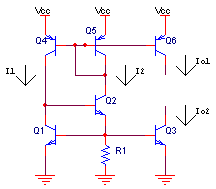
\includegraphics{schematics/self-biasing_Vbe_reference.PNG}
\end{center}
\autocite[311]{analysis-design-analog-ics}

\subsection{Self-biasing $V_{BE}$ reference with startup circuit}
\begin{center}
	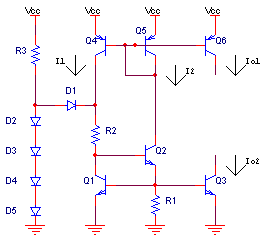
\includegraphics{schematics/self-biasing_Vbe_reference_startup.PNG}
\end{center}
\autocite[312]{analysis-design-analog-ics}

\section{Self-biasing $V_{t}$ reference}
\begin{center}
	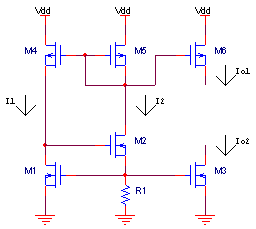
\includegraphics{schematics/self-biasing_Vt_reference.PNG}
\end{center}
\autocite[311]{analysis-design-analog-ics}

\subsection{Self-biasing $V_{t}$ reference with startup circuit}
\begin{center}
	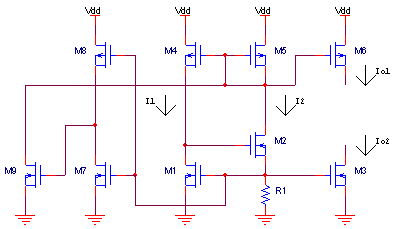
\includegraphics{schematics/self-biasing_Vt_reference_startup.PNG}
\end{center}
\autocite[312]{analysis-design-analog-ics}

%\section{Operational amplifier current regulator (p.231)}

%\section{Operational amplifier boosted output current regulator (p.233)}